%-*- coding: utf-8 -*-
\textcolor[RGB]{46, 116, 181}{\chapter{Initialisation}}
Quelle que soit l’importance des avancées scientifiques et technologiques, c’est le travail des
professionnels de santé qui détermine la qualité et l’efficacité des soins. Dans ce contexte, les soins
nutritionnels, qui portent sur l’évaluation de l’état nutritionnel et l’accompagnement alimentaire des
patients hospitalisés, en interaction étroite avec l’équipe de soin, ne font pas exception. Pour ce
faire, les diététiciens développent des actions de complexité variable, tant au niveau des services de
soins que du système de restauration.

Simultanément, les professionnels doivent faire face à de nouveaux défis, dus aux modifications des
profils épidémiologiques, démographiques et sociaux des populations, ce qui exige la mise en place
de nouvelles compétences et la reconfiguration des stratégies d’action. Pour les diététiciens du
secteur hospitalier, elles ont pour conséquences de nouvelles exigences mentales et surtout
cognitives.

Le niveau de développement industriel de la filière alimentaire française allège la charge de travail
technique des diététiciens, non seulement en ce qui concerne la diversité de matières premières,
mais également dans le domaine du contrôle \enquote{qualité}, tout au long de la chaîne de production. De
la même façon, les nouveaux concepts de production en restauration collective, caractérisés par
l’utilisation de produits pré élaborés et l’innovation technologique des équipements, gagnent
visiblement du terrain dans le secteur hospitalier français.

\section{Définition du problème}
L'élaboration de menus dans un hôpital pour la restauration des patients
est une tâche complexe, et doit tenir compte des différentes pathologies
rencontrées. Faute de moyens (temps et argent) seules quelques grandes
lignes de restauration sont retenues; alors qu'idéalement, chaque
patient devrait pourvoir avoir un repas adapté à sa pathologie.

\section{Vision du projet}
\subsection{Solution envisagée}
Le projet Vitameal a pour objectif de faire correspondre au mieux la planification des régimes et des
prescriptions diététiques aux repas réellement servis au patient. Il consiste en un outil interfaçant la
gestion de production, la prise de commande et le suivi nutritionnel des repas.

\subsection{Périmètre}
C'est un diététicien qui renseigne le profil diététique des patients,
sous les directives des médecins. C'est aussi un diététicien qui élabore
les menus des patients. L'outil permettra donc au diététicien d'élaborer
les menus par filtrage des produits correspondants aux profils
diététiques des patients.
\begin{figure}[H]
\label{Modelisation_du _probleme}
  \centering
      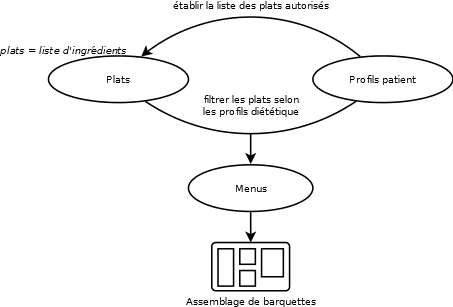
\includegraphics[width=0.75\textwidth]{problem_model} %
\caption{Modélisation du  problème}
\end{figure}

\section{Analyse des exigences}
\subsection{Partie prenantes}
\begin{itemize}
\item Participantes~: les diététiciens, le service restauration
\item Concernés~: les médecins, la direction (budget)
\item Impactées~: les patients
\end{itemize}

\subsection{Les besoins}
\begin{itemize}
\item Les diététiciens renseignent les profils diététiques de chaque patient.
\item Les diététiciens élaborent les menus.
\item Le service restauration commande les produits et ingrédients mis en œuvre dans les menus
\item Le service restauration prépare les menus élaborés.
\item Chaque patient aura une quantité d'aliment correspondante au grammage de l'aliment pour sa tranche d'age (Document \ref{docNutrition}, Annexe 2).
\item La fréquence de service de chaque aliment sera conforme aux recommendations du document de nutrition \ref{docNutrition}, Annexe 4.
\item Chaque aliment devra être classé dans une des catégories d'aliments cité dans les tables de grammages et les fréquences de services du document \ref{docNutrition} Annexes 2 et 4.
\end{itemize}

\subsection{Les contraintes}
\begin{itemize}
\item Les médecins doivent pouvoir vérifier / valider les profils diététiques des patients.
\item La direction fixe un budget maximum par menu.
\end{itemize}

\subsection{Exigences}
\begin{itemize}
\item Fonctionnelles
  \begin{itemize}
  \item Chaque patient a un profil diététique, renseigné par le diététicien
  \item Elaboration automatique des menus, correspondants à un ou plusieurs profils diététiques patients.
  \item À l'issue de l'élaboration des menus, la liste des produits et
    ingrédients (avec leur quantité) est faite afin que le service
    restauration puisse les commander.
  \item La liste des différents menus à réaliser (tickets patients), avec les quantités, est mise à disposition du service restauration pour faciliter l'assemblage du plateau repas.
  \item Ajout de plats.
  \item Chaque plat est décrit avec sa liste d'ingrédients, et la quantité nécessaire à sa réalisation par quantité de poids
  \item Planification des repas par cycles de X semaines
  \end{itemize}
%\item Non fonctionnelles
%  \begin{itemize}
%  \item \colorbox{yellow}{À évaluer !}
%  \end{itemize}
\end{itemize}

\section{\colorbox{yellow}{TODO} Estimation globale}
